\section{Theorie}
\label{sec:Theorie}

\cite{sample}

\subsection{Grundlagen des Photoeffektes}
Der Photoeffekt lässt sich nur schlüssig erklären, wenn Licht durch das Korpuskelmodell beschrieben wird.
Mit monochromatischem Licht wird eine Festkörperoberfläche bestrahlt. Die einzelnen Photonen
übertragen ihre Energie auf die Elektronen in der Festkörperoberfläche. Die Energie
teilt sich in die Austrittsarbeit $A_k$ und die kinetische Energie $E_{kin}$ der Elektronen auf.
Die Austrittsarbeit ist die nötige Energie um ein Elektron aus der Oberfläche zu lösen.

\begin{figure}[H]
  \centering
  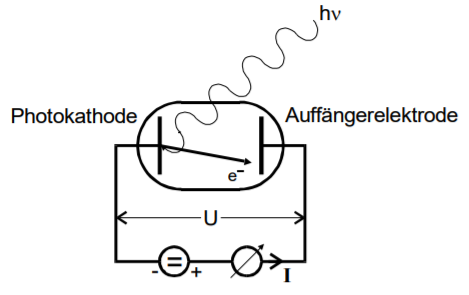
\includegraphics[height=8cm]{anordnung.PNG}
  \caption{Grundlegender Aufbau zur Untersuchung des Photoeffektes. \cite{sample}}
  \label{fig:kathode}
\end{figure}

Hinter der Festkörperoberfläche befindet sich eine Metallplatte, welche in Bezug auf
die Photokathode ein positives Potenzial besitzt. Treffen Elektronen auf diese Platte
kann ein Strom gemessen werden.

Die Photonen haben die Engergie
\begin{align}
  E = h \nu.
\end{align}

Da sich diese Energie beim Auslösen der Elektronen auf $A_k$ und $E_kin$ aufteilt, gilt:
\begin{align}
  h \nu = E_kin + A_k
\end{align}

Ist die Energie der Photonen kleiner als die Austrittsarbeit kann kein Elektronen ausgelöst werden und
es fließt kein Strom, weshalb es eine Grenzfrequenz geben muss, die diesen Fall beschreibt.

Gleichung (2) zeigt außerdem, dass die kinetische Energie ausschließlich proportional zur Frequenz des Lichtes ist.

\subsection{Experimentelle Methode zur Untersuchung des Photoeffektes}

\begin{figure}[H]
  \centering
  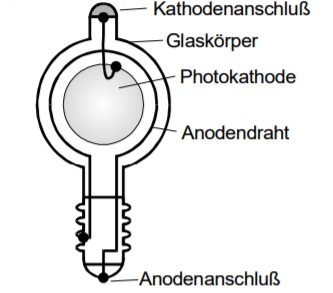
\includegraphics[height=8cm]{photozelle.PNG}
  \caption{Aufbau einer Photozelle. \cite{sample}}
  \label{fig:kathode}
\end{figure}

In einer Photozelle werden Elektronen ausgelöst. Sie besteht aus einer Photokathode, welche mit Licht bestrhlt werden kann.
Diese besteht im Innern aus einer aufgedampften Metall- oder Legierungsschicht.
Die Anode ist ein kreisförmiger Drahtring, welche prallel zur Kathodenoberfläche angebracht ist.

Um die Energie der ausgelösten Elektronen zu bestimmen wird die Gegenfeldmethode verwendet.


\begin{figure}[H]
  \centering
  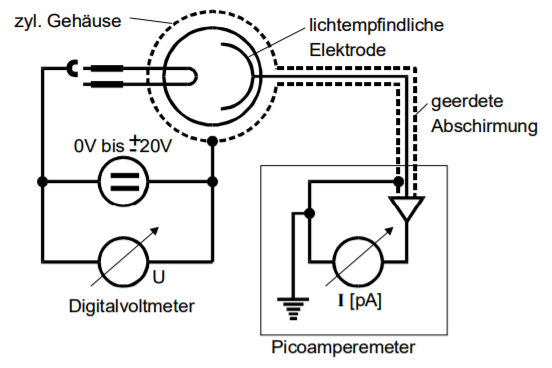
\includegraphics[height=8cm]{gegenfeld.PNG}
  \caption{Messapparatur für die Gegenfeldmethode. \cite{sample}}
  \label{fig:kathode}
\end{figure}

An die Kathoden-Anoden-Strecke wird eine variable Spannung $U$ angelegt. Diese wird so stark eingestellt, sodass die
schnellsten Elektronen gerade nicht die Anode erreichen. Dann entspricht die Energie des Gegenfeldes gerade die der Elektronen.
\begin{align}
  e_0 U_g = \frac{1}{2} m_0 v_{max}^2
\end{align}

Dabei ist $e_0$ die Elementarladung, $v_{max}$ die maximale Geschwindigkeit der Elektronen und $U_g$ die dafür nötige
Spannung des Gegenfeldes.

Dann gilt für die Energie der schnellsten Elektronen:
\begin{equation}
  h \nu = e_0 U_g  + A_k
\end{equation}

Bei der praktischen Durchführung verschwindet der Photostrom jedoch nicht schlagartig bei der Grenzspannung, sondern schon
bei geringeren Spannungen deutlich. Der Grunddafür ist, dass die Elektronen nicht monoenergetisch sind, sondern eine
Energieverteilung von $0$ bis $\frac{1}{2} m v_{max}^2s$ besitzen.
Die Strom-Spannungs-Kurve ist in Abbildung 4 dargestellt.

\begin{figure}[H]
  \centering
  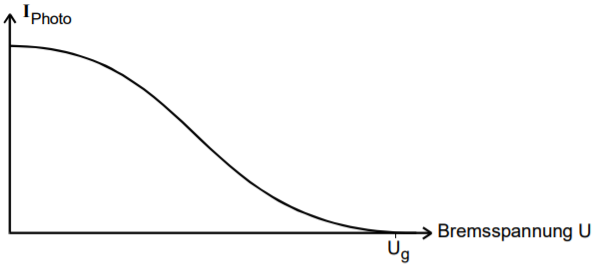
\includegraphics[height=7cm]{fermi.PNG}
  \caption{Photostrom in Abhängigkeit von der Bremsspannung. \cite{sample}}
  \label{fig:kathode}
\end{figure}

Unter bestimmten Vorraussetzungen gibt es zwischen dem Photostrom $I_{Ph}$ und der Bremspannung einen parabolischen Zusammenhang.
\begin{align*}
  I_{Ph} \propto U^2
\end{align*}


Hat das Anodenmaterial eine hohe Austrittsarbeit $A_A$ so können Elektronen, welche zwar ausgelöst werden nicht die
Anode erreichen, falls ihre Energie kleiner als $A_A$ ist. Wird ein beschleunigendes Potential $U_b$ angelegt, können
die Elektronen die Anode wieder erreichen, wenn gilt:
\begin{equation}
  h \nu + e_0 U_b \geq A_A
\end{equation}
